\section{Introduction}

In modern computer architecture design, the storage of instruction and data
follows a hierarchical arrangement called \textbf{memory
hierarchy}, which takes advantage of the access locality and the performance-capacity trade-offs of
diverse memory technologies. The importance of the memory hierarchy
increases with the advances in microprocessor performance~\cite{ITRS07}.
Figure 1 illustrates a typical memory hierarchy. The closer the memory is placed to microprocessor,
the faster latency and higher bandwidth are required, with the penalty of the smaller capacity.
Different memory technologies, such as SRAM, DRAM, and magnetic hard disk drives (HDD) are
the common memory embodiments at the different levels in the memory hierarchy, respectively.
With the improvements in speed, density, and cost of Flash memory,
solid-state drives (SSD) have gained the momentum as the replacements
of the traditional magnetic HDD (Figure 1).

Besides increasing leakage power dissipation, technology scaling also significantly degrades
the reliability of SRAM and DRAM. In recent years, we have seen a lot of efforts have been made
to address the research and development of some
\textbf{emerging non-volatile memory (NVM) technologies}, e.g.,
\textit{Phase-Change RAM (PCRAM)}, \textit{Magnetic RAM (MRAM)}, \textit{Resistive RAM (RRAM)}, and \textit{Memristor}.
By combing the speed of SRAM, the density of DRAM, and the
non-volatility of Flash memory, these emerging memory technologies demonstrated
a great potential to be the candidates of the future universal memories.

In order to enable the massive production and to accelerate the commercialization of the emerging memory technologies,
it is important for designers to understand their physical mechanisms, investigate new circuitries, and look for new
applications for better utilizing them to improve the performance/power/reliability of future computing systems.
To be more specific, we are trying to answer the questions as follows.

Here, we propose a three-year project. The main objective of the proposal is to study design techniques and system
applications for such emerging memory technologies ini future computer systems. The proposed program makes the
following major contributions.
\vspace{5pt}
\squishlist
\item {\textbf{Developing device \underline{models} for emerging non-volatile memories (NVMs):} The device models for emerging non-volatile memories (NVMs) will be developed to fill the gap between process development and circuit design society.}
\item {\textbf{Proposing novel \underline{circuits} techniques:} Based on the unique device characteristics of NVMs, the proposed circuit design techniques could make up the
shortfalls of NVMs and even utilize its advantages. }
\item {\textbf{Exploring novel \underline{applications} on system:} The novel application of the emerging NVM in computing systems will be exploited. The corresponding circuit support and architecture implementation will be investigated too.}
\item {\textbf{Integrated educational plan:} The educational plan will enhance the existing standard curricula by integrating
new course modules on emerging non-volatile memories to complement and upgrade the core computer architecture courses,
and bring the awareness of emerging memory technologies into the circuit design and computer architecture community through
tutorials and workshops.}
\squishend
\vspace{5pt}

\begin{figure}%[htpb]
\centering 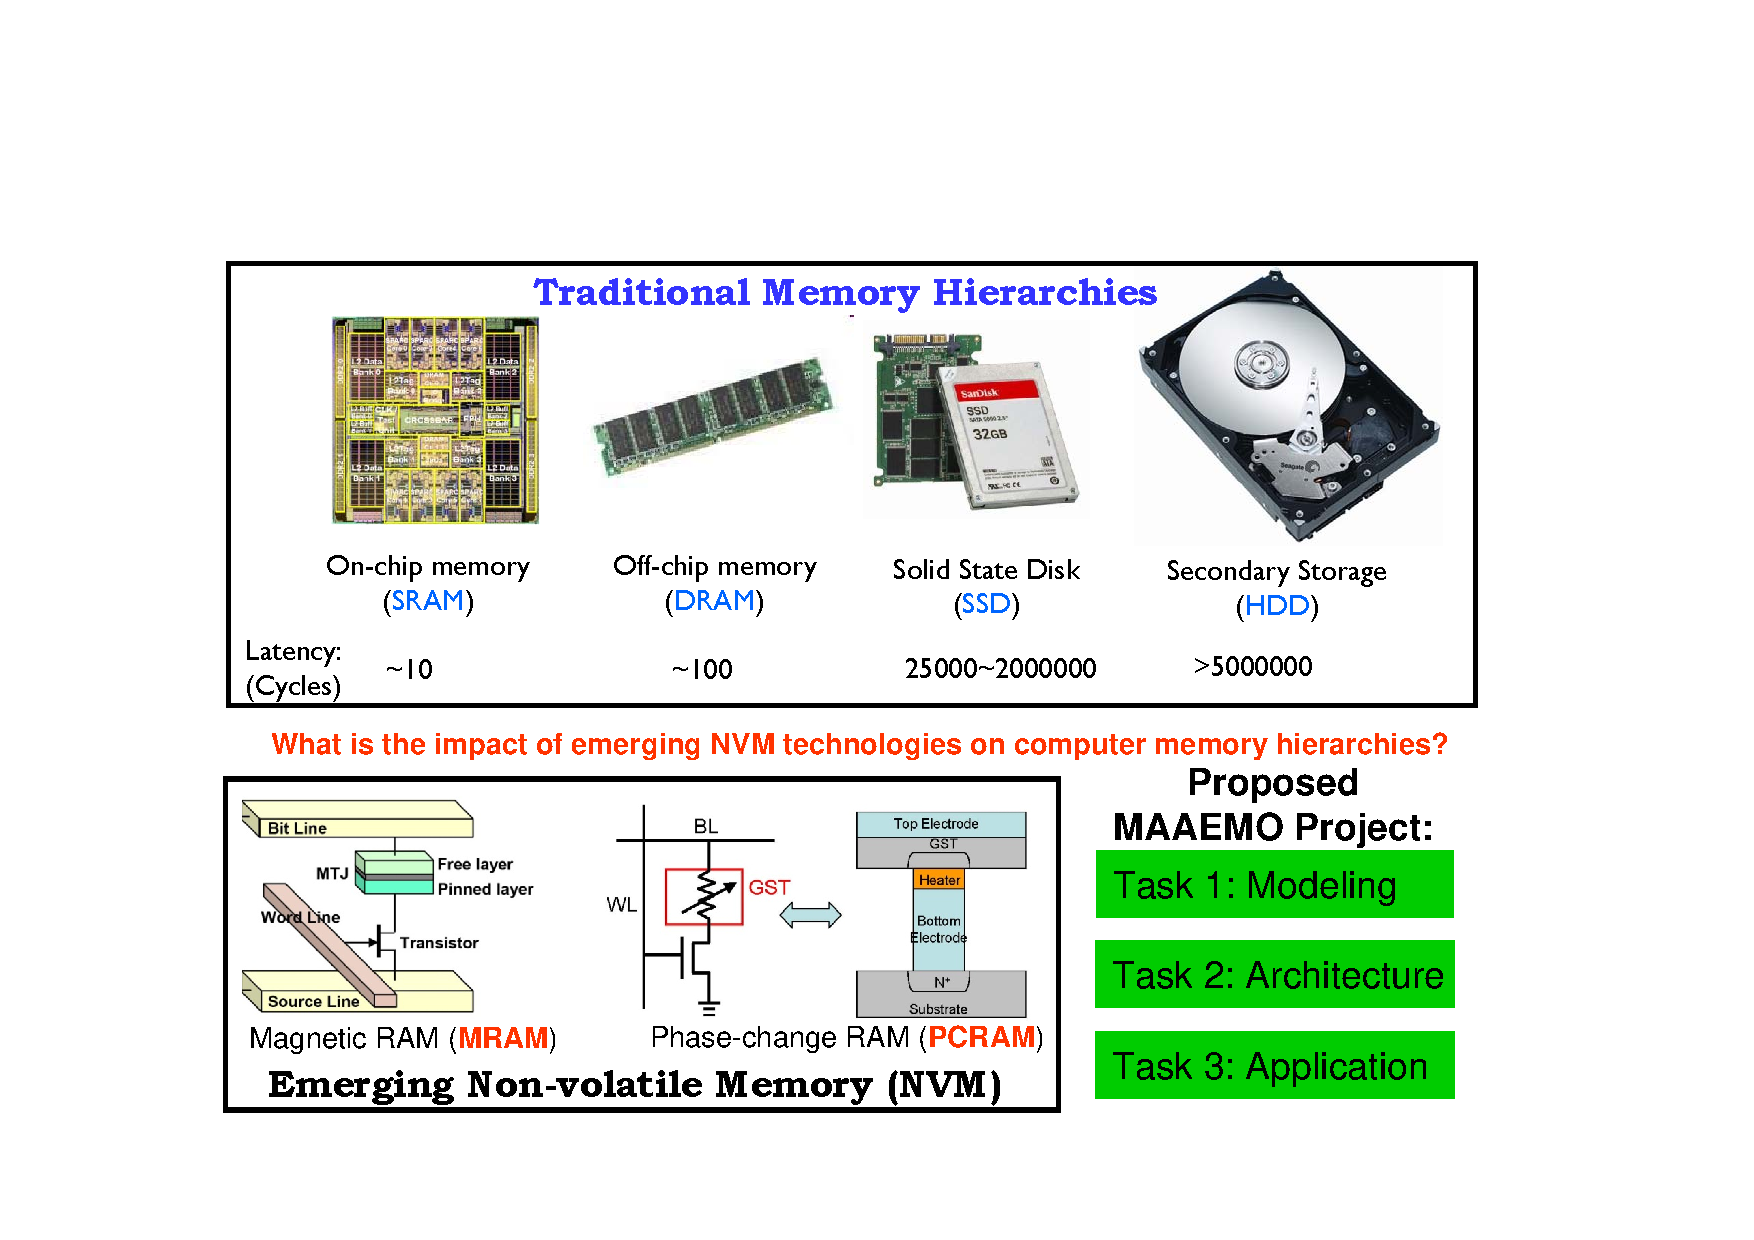
\includegraphics[width=0.8\textwidth]{./figure/mem-hierarchy.pdf}    \vspace{-10pt}
\caption{\textbf{Project Overview.} \underline{Top:} Traditional memory hierarchies consist of SRAM, DRAM, SSD, and HDD; \underline{Bottom:} MRAM and PCRAM are the most promising emerging memory technologies.  \underline{Research Goal:} Study the impact of emerging nonvolatile memory technologies on computer architecture design, with 3 proposed tasks in NVM modeling, architectures, and applications. }\label{mem-hierarchy} \vspace{-10pt}
\end{figure}


Figure 1 illustrates the overview of the proposed project. The proposed work will initiate a novel research direction in high-performance system design and investigate the impact of emerging memory technologies on future computing systems. This work will support the deployment of modern microprocessor designs that use  emerging nonvolatile memory technologies. The proposed research will provide a complementary perspective to the existing computing system research.


\begin{comment}
As such emerging memory technologies are getting mature, it is important for architecture
designers to understand their pros and cons for better utilizing them to improve
the performance/power/reliability of future computing systems.
To be more specific, we are trying to answer the questions as follows.

 \vspace{5pt}
\begin{tabular}{|l|}
\hline
$\bullet$ \textit{How to model such emerging NVM technologies?} \\
$\bullet$ \textit{What will be the impacts of such NVMs on the future memory hierarchy?}\\
$\bullet$ \textit{What are the research challenges to overcome for such a new memory hierarchy?} \\
$\bullet$ \textit{What will be the novel applications/architectures with emerging NVM technologies?} \\
$\bullet$ \textit{How can graduate students be prepared for such future novel architectural innovations?}  \\
\hline
\end{tabular} \vspace{5pt}

    To answer these questions, we propose a three-year project. The main objective of the proposal is to study the design implication of such emerging memory technologies for future computer architecture systems. The proposed program makes the
following major contributions.


%\squishlistindent
\squishlist
\item {\textbf{Task 1:} Developing \textbf{models} for emerging non-volatile memories (NVMs).}
\item {\textbf{Task 2:} Proposing novel memory \textbf{architecture} to leverage emerging NVM technologies.}
\item {\textbf{Task 3:} Exploring novel \textbf{applications} that leverage  emerging NVM technologies.}
\item {\textbf{Integrated educational plan:} Enhancing the core computer architecture courses with new NVM course modules.}
%The educational plan will %enhance the existing standard curricula by integrating new course modules on %nonvolatile memory, with multi-institutional graduate-level course, to %complement and upgrade the core computer architecture courses.}
\squishend

\end{comment}
